\documentclass[10pt,a4paper,twoside,openright]{report}

\usepackage[default]{lato}
\usepackage{inconsolata}
\usepackage[T1]{fontenc}
\usepackage[utf8]{inputenc}
\usepackage[english,dutch]{babel}
\usepackage[chapter]{minted}
\usepackage{a4wide}
\usepackage[font=small,format=plain,labelfont=bf,up,textfont=it,up]{caption}
\usepackage{xcolor}
\usepackage{graphicx}
\usepackage[pdftex]{hyperref}
\usepackage[inline]{enumitem}
\usepackage{amsmath}
\usepackage{units}

\usepackage[toc,page]{appendix}
\renewcommand{\appendixname}{Bijlagen}
\renewcommand{\appendixtocname}{Bijlagen}
\renewcommand{\appendixpagename}{Bijlagen}

\usepackage{tikz}
\usetikzlibrary{trees}
\usetikzlibrary{decorations}
\usetikzlibrary{arrows,positioning,shapes}
\usetikzlibrary{calc}
\usetikzlibrary{decorations.markings}
\usetikzlibrary{automata}

\newcommand{\code}[1]{\textbf{\texttt{#1}}}

\hypersetup{pdftitle={Autonerf}}

\begin{document}
    \include{figures/setup}

    \usemintedstyle{github}
    \newminted{cpp}{gobble=4,linenos,fontsize=\small,bgcolor=black!5}
    \newminted{json}{gobble=4,linenos,fontsize=\small,bgcolor=black!5}

    \begin{titlepage}

\Huge \textsc{\bfseries \autonerf} \normalsize \\

\vfill

\begin{minipage}[b][1em][b]{\linewidth}
    Hogeschool van Arnhem en Nijmegen, Ruitenberglaan 26 te Arnhem
\end{minipage}

\begin{minipage}[b][2em][b]{\linewidth}
\end{minipage}

\begin{minipage}[b][4em][b]{\linewidth}
    \begin{tabular}{l l }
        Projectgroep: & Ramon Kleiss \texttt{<ramonkleiss@gmail.com>} \\
        & Niek van der Straaten \texttt{<niekvds@gmail.com>} \\
        \\
        Begeleider: & Hugo Arends \texttt{<hugo.arends@han.nl>} \\
    \end{tabular}
\end{minipage}

\end{titlepage}


    \tableofcontents
    \listoffigures

    \chapter{Inleiding}
\label{ch:introduction}

Dit verslag is geschreven in opdracht van de Hogeschool van Arnhem in Nijmegen
(HAN) in het kader van de minor Embedded Vision Design (EVD) aan de opleiding
Embedded Systems Engineering (ESE). Het omschrijft hoe het project van de studenten
is ontwikkeld en waarom bepaalde design keuzes zijn gemaakt gedurende de
ontwikkeling van het product.

Het doel van het project was om een autonome \emph{Nerfgun} (zie figuur \ref{fig:nerf})
te ontwikkelen. Dit product moet in staat zijn om een persoon te herkenning
en er vervolgens een \emph{dart} (figuur \ref{fig:nerfdart}) op af te vuren. De
officiele omschrijving van het project is als volgt:

\begin{quote}
“Uiterlijk week 8 van het academisch jaar 2013/2014 zal een systeem ontwikkeld zijn die
autonoom een Nerfgun kan afvuren op bewegende doelwitten (personen). Het systeem moet
gebruik maken van camera beelden om deze doelwitten te vinden binnen een omgeving.”
\end{quote}

Het systeem is gedoopt tot \emph{Autonerf} (een samenvoeging van \emph{autonoom}
en \emph{Nerf}). In dit verslag worden de resultaten van de verschillende projectfasen besproken
en uitgelegd.

\vfill
\pagebreak

Het eerste deel dat zal worden beschreven is het functioneel ontwerp
(\ref{ch:functional}). Hier zal functioneel beschreven worden \emph{wat} het
systeem moet doen. Er zal verder niet worden ingegaan op \emph{hoe} het systeem
dit bereikt. Het hoofdstuk Technische Specificatie (\ref{ch:technical}) zal hier
verder op ingaan. In hoofdstuk \ref{ch:realization} zal de realisatie van het
project beschrijven. Er zal besproken worden welke beslissingen er gemaakt zijn
en waarom deze gemaakt zijn. Uiteindelijk zullen de resultaten van het testen
(hoofdstuk \ref{ch:testing}) besproken worden. Daarnaast zal in hoofdstuk
\ref{ch:conclusion} een conclusie worden getrokken en zullen eventuele
aanbevelingen worden gedaan voor het doorontwikkelen van het product.

\begin{figure}[H]
    \begin{minipage}{0.45\textwidth}
        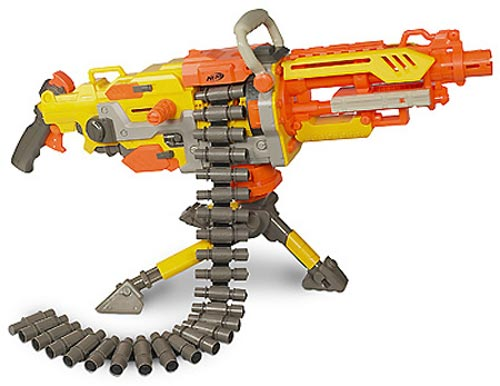
\includegraphics[width=\linewidth]{figures/nerfgun.jpg}
        \caption{Een Nerfgun}
        \label{fig:nerf}
    \end{minipage}
    \begin{minipage}{0.45\textwidth}
        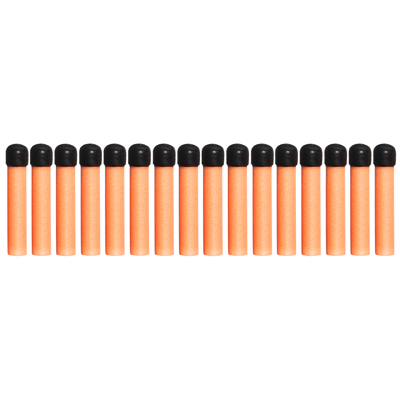
\includegraphics[scale=.5,width=\linewidth]{figures/nerfdart.png}
        \caption{Een Nerf dart}
        \label{fig:nerfdart}
    \end{minipage}
\end{figure}

    \chapter{Functioneel Ontwerp}
\label{ch:functional}

Dit hoofdstuk definiëerd de functionele specificatie van het Autonerf project.
Het beschrijft een aantaal functionele eisen en de functionele architectuur
van het systeem.

\section{Specificatie}

Het te ontwikkelen systeem moet aan de volgende eisen voldoen:

\begin{itemize}
    \item Het systeem moet kunnen werken op een gewone computer;
    \item Het systeem moet personen herkennen en daar \emph{darts} op af vuren;
    \item Het systeem moet (om personen te herkennen) gebruik maken van
        real-time camera beelden;
    \item Het systeem moet in staat zijn op bewegende doelwitten te kunnen vuren.
\end{itemize}

\section{Architectuur}
\label{sec:func:arch}

De omschrijving van de architectuur van het Autonerf systeem begint bij het
globale input-proces-output (IPO) schema (te zien in figuur \ref{fig:global-ipo}).
Dit schema toont de inputs van het systeem (de real-time camera beelden) en de
output van het systeem (de dart die mogelijk afgevuurd wordt).

\begin{figure}[H]
    \begin{center}
        \begin{tikzpicture}[font=\sffamily,
  every matrix/.style={ampersand replacement=\&,column sep=1cm,row sep=1cm},
  source/.style={inner sep=.3cm},
  process/.style={draw,thick,rounded corners,fill=yellow!10,inner sep=.3cm},
  sink/.style={source},
  datastore/.style={draw,very thick,shape=datastore,inner sep=.3cm},
  dots/.style={gray,scale=2},
  to/.style={->,>=stealth',shorten >=1pt,thick,font=\sffamily\footnotesize},
  every node/.style={align=center,font=\footnotesize}]

    \matrix {
        \node[source](in){Real-time camera beelden};
            \& \node[process](proc){Verwerken camera beelden};
            \& \node[sink](out){Commando's Nerfgun}; \\
    };

    \draw[to](in) -- (proc);
    \draw[to](proc) -- (out);
\end{tikzpicture}

    \end{center}
    \caption{Het globale input-process-output schema van het Autonerf systeem}
    \label{fig:global-ipo}
\end{figure}

\vfill
\pagebreak

Om de taak goed te kunnen uitvoeren heeft het systeem de volgende logische
blokken nodig:

\begin{enumerate}
    \item De \emph{reader}: verantwoordelijk is voor de acquisitie van
        frames vanuit de real-time feed van de camera beelden;
    \item De \emph{detector}: verantwoordelijk voor het detecteren van gezichten
        in een frame;
    \item De \emph{recognizer}: verantwoordelijk voor het herkennen van gezichten
        en deze aan bepaalde personenen koppelen zodat hiermee een conclusie
        uit kan worden getrokken;
    \item De \emph{localizer}: verantwoordelijk voor het bepalen van de locatie
        en radiale afwijking van gezichten op basis van ontvangen frames;
    \item De \emph{controller}: verantwoordelijk voor het aansturen van de
        Nerfgun.
\end{enumerate}

\begin{figure}[H]
    \begin{center}
        \begin{tikzpicture}[font=\sffamily,
  every matrix/.style={ampersand replacement=\&,column sep=1cm,row sep=1cm},
  source/.style={inner sep=.3cm},
  process/.style={draw,thick,rounded corners,fill=yellow!10,inner sep=.3cm},
  sink/.style={source},
  datastore/.style={draw,very thick,shape=datastore,inner sep=.3cm},
  dots/.style={gray,scale=2},
  to/.style={->,>=stealth',shorten >=1pt,thick,font=\sffamily\footnotesize},
  every node/.style={align=center,font=\footnotesize}]

    \matrix {
        \node[process](read){Reader};
            \& \node[process](detect){Detector};
            \& \node[process](local){Localizer};
            \& \node[process](control){Controller}; \\
    };

    \draw[to](read) -- (detect);
    \draw[to](detect) -- (local);
    \draw[to](local) -- (control);
\end{tikzpicture}

    \end{center}
    \caption{De logische blokken van het Autonerf systeem}
    \label{fig:func-architecture}
\end{figure}

    \chapter{Technisch Ontwerp}
\label{ch:technical}

\section{Hierarchie}

Zoals beschreven kan de architectuur van het systeem (sectie \ref{sec:func:arch})
opgedeeld worden in zes logische blokken:

\begin{enumerate}
    \item De \emph{reader}
    \item De \emph{detector}
    \item De \emph{recognizer}
    \item De \emph{localizer}
    \item De \emph{controller}
\end{enumerate}

Deze logische blokken kunnen worden opgedeeld in een aantal sub-blokken. De
hierarchie van deze sub-blokken is te zien in figuur \ref{fig:hierarchy}.

\begin{figure}[H]
    % \begin{center}
        \begin{tikzpicture}[font=\sffamily,
  every matrix/.style={ampersand replacement=\&,column sep=.25cm,row sep=1cm},
  source/.style={inner sep=.3cm},
  process/.style={draw,thick,rounded corners,fill=yellow!10,inner sep=.3cm},
  sink/.style={source},
  datastore/.style={draw,very thick,shape=datastore,inner sep=.3cm},
  dots/.style={gray,scale=2},
  to/.style={>=stealth',shorten >=1pt,thick,font=\sffamily\footnotesize},
  sub/.style={->,to},
  every node/.style={align=center,font=\footnotesize}]

    \matrix {
        \node[process](reader){Reader};
            \& \& \node[process](detector){Detector};
            \& \& \node[process](localizer){Localizer};
            \& \& \node[process](controller){Controller}; \\

        \& \& \& \node[process](enhance){Enhancer}; \\
        \& \& \& \node[process](seg1){Segmentator}; \\
        \& \& \& \node[process](extr1){Feature extractor}; \\
        \& \& \& \node[process](class1){Classifier}; \\
    };

    \draw[to](reader) -- (detector);
    \draw[to](detector) -- (localizer);
    \draw[to](localizer) -- (controller);

    \draw[sub](detector) |- (enhance);
    \draw[sub](detector) |- (seg1);
    \draw[sub](detector) |- (extr1);
    \draw[sub](detector) |- (class1);
\end{tikzpicture}

    % \end{center}
    \caption{De hierarchie van het Autonerf systeem}
    \label{fig:hierarchy}
\end{figure}

\section{Architectuur}

De data-flow van het systeem begint bij het \emph{reader} subsysteem. Dit subsysteem
is verantwoordelijk voor het uitlezen van de camera en het verkrijgen van individuele
frames vanuit de camera. Dit systeem stuurt de uitgelezen frames door naar het
\emph{detector} subsysteem die probeert gezichten te detecteren in het systeem.
Als dit gelukt is en een gezicht gedetecteerd is word de data doorgestuurd naar
de \emph{recognizer} en \emph{localizer} subsystemen. Het \emph{recognizer}
subsysteem probeert het gedetecteerde gezicht te herkennen. Als een gezicht
herkend wordt, wordt dit doorgegeven aan het \emph{controller} subsysteem.
Het \emph{localizer} subsysteem berekend de locatie van het gezicht en de afwijking
ervan tot het centrum van het frame (met eventueel een bepaalde toegestane
\emph{offset}). Het \emph{controller} subsysteem is uiteindelijk verantwoordelijk
voor de aansturing van de Nerfgun.

\subsection{De \emph{reader}}

Zoals getoont in figuur \ref{fig:ipo-reader} heeft het \emph{reader} subsysteem
maar één input en output: de frames van de camera. Dit gebeurd door middel van
een USB-verbinding met de camera. Het \emph{reader} subsysteem vervult de rol
van de \emph{Acquisition} stap binnen het vision-model.

De output van het systeem is een RGB frame van 640 $\times$ 480 pixels wat wordt
opgeslagen in een matrix. Deze matrix is de output van het systeem.

\begin{figure}[H]
    \begin{center}
        \begin{tikzpicture}[font=\sffamily,
  every matrix/.style={ampersand replacement=\&,column sep=1cm,row sep=2cm},
  source/.style={inner sep=.3cm},
  process/.style={draw,thick,rounded corners,fill=yellow!10,inner sep=.3cm},
  sink/.style={source},
  datastore/.style={draw,very thick,shape=datastore,inner sep=.3cm},
  dots/.style={gray,scale=2},
  to/.style={->,>=stealth',shorten >=1pt,thick,font=\sffamily\footnotesize},
  every node/.style={align=center,font=\footnotesize}]

    \matrix {
        \node[source](in){Frame van USB-camera};
            \& \node[process](proc)[]{Uitlezen frames van USB-camera};
            \&  \node[sink](out)[]{Uitgelezen frame}; \\
    };

    \draw[to](in) -- (proc);
    \draw[to](proc) -- (out);
\end{tikzpicture}

    \end{center}
    \caption{Het IPO-schema van het \emph{reader} subsysteem}
    \label{fig:ipo-reader}
\end{figure}

\subsection{De \emph{detector}}

Het IPO-schema van het \emph{detector} subsysteem (figuur \ref{fig:ipo-detector})
heeft één input en output. De input van het systeem is het uitgelezen frame van
de camera (de eerder genoemde frame). De outputs zijn eventueel gedetecteerde gezichten en het originele
frame dat ontvangen is. Als er geen gezicht gedetecteerd wordt stopt de data-stroom
in dit systeem. Binnen het vision-model vervult de \emph{detection} de
stappen \emph{enhancement}, \emph{segmentation}, \emph{feature extraction} en
\emph{classification}.

\begin{figure}[H]
    \begin{center}
        \begin{tikzpicture}[font=\sffamily,
  every matrix/.style={ampersand replacement=\&,column sep=1cm,row sep=1cm},
  source/.style={inner sep=.3cm},
  process/.style={draw,thick,rounded corners,fill=yellow!10,inner sep=.3cm},
  sink/.style={source},
  datastore/.style={draw,very thick,shape=datastore,inner sep=.3cm},
  dots/.style={gray,scale=2},
  to/.style={->,>=stealth',shorten >=1pt,thick,font=\sffamily\footnotesize},
  every node/.style={align=center,font=\footnotesize}]

    \matrix {
        \& \& \node[sink](out1)[]{Uitgelezen frame}; \\

        \node[source](in){Uitgelezen frame};
            \& \node[process](proc)[]{Detecteren gezichten in frame}; \\

        \& \& \node[sink](out2)[]{Gedetecteerde gezichten}; \\
    };

    \draw[to](in) -- (proc);
    \draw[to](proc) |- (out1);
    \draw[to](proc) |- (out2);
\end{tikzpicture}

    \end{center}
    \caption{Het IPO-schema van het \emph{detector} subsysteem}
    \label{fig:ipo-detector}
\end{figure}

De subsystemen van het \emph{detector} subsysteem zijn de \emph{enhancer},
\emph{segmentator}, \emph{feature extractor} en \emph{classifier} systemen.

\subsubsection{Enhancer}

Het enhancer subsubsysteem krijgt als input het frame wat is uitgelezen door
het \emph{reader} systeem. Allereerst wordt dit frame geconverteerd naar een
grayscale beeld. Daarna wordt er \emph{histogram equalization} uitgevoerd
waardoor de gezichtdetectie accurater wordt.

\subsubsection{Segmentator}

Het \emph{segmentator} subsysteem heeft als input
het verbeterde frame van het \emph{enhancer} subsubsysteem. De pixels in dit
frame worden vergeleken door middel van integratie. De uitkomst van deze
vergelijking wordt opgeslagen in een matrix die de output van het systeem is.

\subsubsection{Feature extractor}

Als input verwacht het \emph{feature extractor} subsysteem het gesegmenteerde
frame van het \emph{segmentator} subsysteem. Deze matrix wordt gecontroleerd
op bepaalde \emph{Haar-features}. De output van het systeem is een overzicht
van welke features waar in het frame aanwezig zijn.

\subsubsection{Classifier}

Als input verwacht het \emph{classifier} subsysteem de output van het \emph{feature
extractor} subsysteem. De \emph{Haar Classifier} beslist op basis van het aantal
en de verdeling van de Haar features of er sprake is van een gezicht of niet.
De output zijn de coordinaten van de gedetecteerde gezichten.

\subsection{De \emph{recognizer}}

Het \emph{recognizer} subsysteem (figuur \ref{fig:ipo-recognizer}) heeft als
inputs:

\begin{enumerate}
    \item De coordinaten van gedetecteerde gezichten;
    \item en het frame ontvangen door het \emph{detector} subsysteem.
\end{enumerate}

Als output heeft het subsysteem een persoon wat eventueel herkend is. Als er
geen persoon herkend is in het frame heeft het systeem geen verdere outputs.
Het systeem vervult, net als het \emph{detector} subsysteem de stappen \emph{segmentation},
\emph{feature extraction} en \emph{classification} binnen het vision-model. Er
zijn dan ook dezelfde subsystem aanwezig als binnen het \emph{detector} subsysteem.

\begin{figure}[H]
    \begin{center}
        \begin{tikzpicture}[font=\sffamily,
  every matrix/.style={ampersand replacement=\&,column sep=1cm,row sep=1cm},
  source/.style={inner sep=.3cm},
  process/.style={draw,thick,rounded corners,fill=yellow!10,inner sep=.3cm},
  sink/.style={source},
  datastore/.style={draw,very thick,shape=datastore,inner sep=.3cm},
  dots/.style={gray,scale=2},
  to/.style={->,>=stealth',shorten >=1pt,thick,font=\sffamily\footnotesize},
  every node/.style={align=center,font=\footnotesize}]

    \matrix {
        \node[source](in1){Gedetecteerde gezichten};\\

        \& \node[process](proc){Herkennen personen};
            \& \node[sink](out){Herkende personen}; \\

        \node[source](in2){Ontvangen frame}; \\
    };

    \draw[to](in1) -| (proc);
    \draw[to](in2) -| (proc);
    \draw[to](proc) -- (out);
\end{tikzpicture}

    \end{center}
    \caption{Het IPO-schema van het \emph{recognizer} subsysteem}
    \label{fig:ipo-recognizer}
\end{figure}

\subsubsection{Segmentator}

De input van het \emph{segmentator} sub-subsysteem is het frame wat verkregen is
door het \emph{reader} subsysteem. Dit systeem maakt gebruik van \emph{Local
Binary Patterns} (LBP) om gezichten te herkennen. Het LBP algoritme vergelijkt
door middel van thresholds elke pixel met zijn \emph{neighbours}. De output
van het \emph{segmentator} systeem is een LBP-matrix waarin elke pixel een
waarde heeft die de lokale structuur van zijn neighbours aangeeft.

\subsubsection{Feature extractor}

De input van het \emph{feature extractor} subsubsysteem is de LBP-matrix die door
het \emph{segmentator} subsysteem berekend wordt. Deze matrix wordt opgedeeld
in lokale regio's. Van deze regio's wordt een histogram gemaakt die vervolgens
gelinkt in een matrix worden geplaatst waardoor de features in alle regio's
zichtbaar zijn. Deze histogram-matrix is de output van het \emph{feature
extractor} subsubsysteem.

\subsubsection{Classifier}

De input van het \emph{classifier} sub-subsysteem is de histogram-matrix output
van het \emph{segmentator} sub-subsysteem. Deze matrix wordt vergeleken met matrixes
van foto's uit de gezichten database. Op basis van overeenkomsten wordt bepaald
of de gezichten van dezelfde persoon zijn. De output van het systeem is een
voorspeld label (elk persoon heeft in de database zijn eigen label).

\subsection{De \emph{localizer}}

Zoals te zien in figuur \ref{fig:ipo-localizer} heeft het \emph{localizer}
subsysteem twee inputs: de coordinaten van eventueel herkende gezichten en
het frame dat ontvangen is door het \emph{detector} subsysteem. De output
van het systeem zijn de ruimtelijke coordinaten van de gedetecteerde gezichten
ten opzichte van het centrum van het frame (de origin).

\begin{figure}[H]
    \begin{center}
        \begin{tikzpicture}[font=\sffamily,
  every matrix/.style={ampersand replacement=\&,column sep=1cm,row sep=1cm},
  source/.style={inner sep=.3cm},
  process/.style={draw,thick,rounded corners,fill=yellow!10,inner sep=.3cm},
  sink/.style={source},
  datastore/.style={draw,very thick,shape=datastore,inner sep=.3cm},
  dots/.style={gray,scale=2},
  to/.style={->,>=stealth',shorten >=1pt,thick,font=\sffamily\footnotesize},
  every node/.style={align=center,font=\footnotesize}]

    \matrix {
        \node[source](in1){Gedetecteerde gezichten};\\

        \& \node[process](proc){Lokaliseren gezichten};
            \& \node[sink](out){Ruimtelijke coordinaten}; \\

        \node[source](in2){Ontvangen frame}; \\
    };

    \draw[to](in1) -| (proc);
    \draw[to](in2) -| (proc);
    \draw[to](proc) -- (out);
\end{tikzpicture}

    \end{center}
    \caption{Het IPO-schema van het \emph{localizer} subsysteem}
    \label{fig:ipo-localizer}
\end{figure}

\subsection{De \emph{controller}}

Het \emph{controller} subsysteem (figuur \ref{fig:ipo-controller}) heeft als inputs:

\begin{enumerate}
    \item Het frame ontvangen door het \emph{detector} subsysteem;
    \item De radiale afwijking van eventueel gedetecteerde gezichten;
    \item en eventueel herkende personen binnen het frame.
\end{enumerate}

Als output heeft het systeem de commando's die naar de Nerfgun gestuurd moeten
worden.

\begin{figure}[H]
    \begin{center}
        \begin{tikzpicture}[font=\sffamily,
  every matrix/.style={ampersand replacement=\&,column sep=1cm,row sep=1cm},
  source/.style={inner sep=.3cm},
  process/.style={draw,thick,rounded corners,fill=yellow!10,inner sep=.3cm},
  sink/.style={source},
  datastore/.style={draw,very thick,shape=datastore,inner sep=.3cm},
  dots/.style={gray,scale=2},
  to/.style={->,>=stealth',shorten >=1pt,thick,font=\sffamily\footnotesize},
  every node/.style={align=center,font=\footnotesize}]

    \matrix {
        \node[source](in1){Herkende personenen};\\

        \& \node[process](proc){Bepalen commando's voor Nerfgun};
            \& \node[sink](out){Commando's voor Nerfgun}; \\

        \node[source](in2){Ruimtelijke coordinaten gezichten}; \\
    };

    \draw[to](in1) -| (proc);
    \draw[to](in2) -| (proc);
    \draw[to](proc) -- (out);
\end{tikzpicture}

    \end{center}
    \caption{Het IPO-schema van het \emph{controller} subsysteem}
    \label{fig:ipo-controller}
\end{figure}

    \chapter{Realisatie}
\label{ch:realization}

\section{Software}

De software van het Autonerf systeem is geïmplementeerd in C++ waarbij gebruikt
wordt gemaakt van de libraries van OpenCV. OpenCV is een groep libraries die
ontwikkeld zijn voor \emph{computer vision} (OpenCV staat dan ook voor
\emph{Open Computer Vision}).

De software is \emph{event driven} geschreven. Dit betekend dat, in plaats dat
er gepolled wordt door object voor data, er met events wordt gewerkt. Wanneer
er binnen een object een event plaatsvindt, worden andere \emph{subscribers}
hier van op de hoogte gebracht.

Events worden met een basisklasse (\code{Autonerf::Emitter}) ge-\emph{emit}.
Objecten kunnen door een handler te registreren (met behulp van de \code{on}
methode) ``luisteren'' voor events.

\subsection{De \emph{reader}}

Voor het uitlezen van de camera beelden door de \code{Reader} klasse wordt
gebruik gemaakt van de OpenCV klasse \code{cv::VideoCapture}. Deze klasse geeft
een \code{cv::Mat} object wat een RGB frame representeerd (zie \ref{ls:reader}).

\begin{listing}[H]
    \begin{cppcode}
    cv::Mat frame;

    if (!this->capture.isOpened()) {
        throw std::runtime_error("Cannot capture frame from closed device.");
    }

    if (!this->capture.grab()) {
        return;
    }

    if (!this->capture.read(frame)) {
        throw std::runtime_error("Could not read frame from capture device.");
    }

    this->emit("frame", json_integer((json_int_t) &frame));
    \end{cppcode}
    \caption{Het uitlezen van een frame van de camera.}
    \label{ls:reader}
\end{listing}

\subsection{De \emph{detector}}

Alle subsystemen van het \emph{detector} subsysteem worden geïmplementeerd door
de OpenCV klasse \code{cv::CascadeClassifier}. Deze klasse maakt gebruik van
Haar cascades om gezichten te detecteren in beelden (zie listing \ref{ls:classifier}).

\begin{listing}[H]
    \begin{cppcode}
    std::vector<cv::Rect> faces;

    this->classifier.detectMultiScale(
        grayscale,
        faces,
        1.1,
        3,
        CV_HAAR_FIND_BIGGEST_OBJECT|CV_HAAR_SCALE_IMAGE,
        cv::Size(50, 50)
    );

    if (face.size() > 0) {
        this->emit(
            "detected",
            // informatie van locatie grootste gezicht in beeld
        );
    }
    \end{cppcode}
    \caption{Het detecteren van gezichten met de \code{cv::CascadeClassifier} klasse}
    \label{ls:classifier}
\end{listing}

\subsubsection{Enhancer}

Het frame wat uitgelezen is door de \emph{reader} klasse wordt geconverteerd
naar een grayscale beeld met behulp van de \code{cv::cvtColor} (zie listing \ref{ls:det-enhc})
method. Dit wordt gedaan omdat de \emph{Segmentator} een grayscale beeld verwacht.
Daarnaast wordt er een \emph{histogram equalization} uitgevoerd. Hiermee wordt
het contrast van het beeld verbeterd waardoor de intensiteit beter verdeeld is.
Door dit te doen worden details in het hele beeld beter zichtbaar, waardoor de
de gezichtsdetectie en -herkenning makkelijker verlopen. Figuur \ref{fig:sinterklaas1}
en \ref{fig:sinterklaas2} laat een voorbeeld zien van deze operatie.

\begin{listing}[H]
    \begin{cppcode}
    cv::cvtColor(frame, grayscale, CV_BGR2GRAY);

    cv::equalizeHist(grayscale, grayscale);
    \end{cppcode}
    \caption{Het \emph{enhancen} van uitgelezen camera beelden}
    \label{ls:det-enhc}
\end{listing}

\begin{figure}[H]
    \begin{minipage}{0.45\textwidth}
        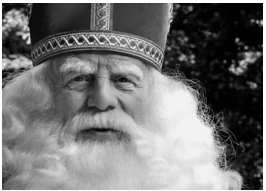
\includegraphics[width=\linewidth]{figures/sint-before.png}
        \caption{Voor \emph{histogram equalization}}
        \label{fig:sinterklaas1}
    \end{minipage}
    \begin{minipage}{0.45\textwidth}
        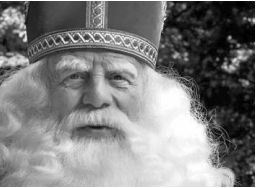
\includegraphics[width=\linewidth]{figures/sint-after.png}
        \caption{Na \emph{histogram equalization}}
        \label{fig:sinterklaas2}
    \end{minipage}
\end{figure}

\subsubsection{Segmentator}

De \emph{segmentator} verzorgt de segmentatie van ontvangen frames. Het hele frame
afgegaan waarbij elke pixel wordt vergeleken met zijn omgeving. De pixel waarden
van de omgeving worden geïntegreerd waarna deze waarde in de pixel wordt gezet
die met zijn omgeving is vergeleken.

\subsubsection{Feature extractor}

Nadat alle pixels zijn geïntegreerd met hun omgeving wordt er gekeken welke Haar
features er aanwezig zijn in het beeld. Dit wordt gedaan door van elke Haar
feature de gemiddelde pixelwaarde van het donkere deel af te trekken van de
gemiddelde pixel waarde van het lichte deel. Als deze waarde boven een bepaalde
threshold ligt wordt er aangenomen dat de Haar feature aanwezig is in de regio
van het beeld waar op dat moment naar wordt gekeken. OpenCV verzorgd standaard
een aantal files die Haar features beschrijven, waaronder één die een gezicht
van de voorkant beschrijft. In het Autonerf systeem wordt dit bestand gebruikt.

\begin{figure}[H]
    \begin{center}
        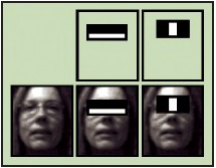
\includegraphics[scale=0.75]{figures/haar-features.png}
        \caption{Haar features in een gezicht}
    \end{center}
\end{figure}

\vfill
\pagebreak

\subsubsection{Classifier}

De door de \emph{feature extractor} beschreven Haar features en thresholds worden
bepaald door een techniek voor \emph{machine-learning} genaamd AdaBoost. Met deze
techniek wordt er per regio gekeken of een door AdaBoost geselecteerde Haar
feature aanwezig is. Als dit niet het geval is wordt de regio direct afgeschreven
als gezicht. Als het wél het geval is gaat de regio door naar de volgende \emph{stage}
en wordt een andere feature geselecteerd, et cetera. Als de regio succesvol alle
\emph{stages} passeert is er sprake van een gezicht.

\begin{figure}[H]
    \begin{center}
        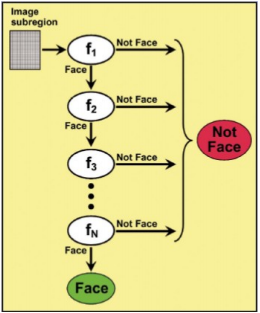
\includegraphics[scale=0.75]{figures/adaboost-classification.png}
        \caption{AdaBoost classificatie}
    \end{center}
\end{figure}

\subsection{De \emph{localizer}}

Het lokaliseren van gezichten is eigenlijk een triviale taak. Zodra de coordinaten
(binnen het frame) bekend zijn van het gezicht, kan hiermee de ruimtelijke
afwijking van het gezicht ten opzichte van het centrum van het frame.

Als we het centrum van het frame $(0, 0)$ dopen, kan de locatie van het gezicht
worden geschreven als $(x, y)$. Een camera heeft een zogenaamd
\emph{field-of-view} (FOV) wat in graden wordt uitegedrukt. Door middel van deze
eigenschap van de camera, kan precies berekend worden hoeveel graden per pixel
er in het frame zitten (zowel horizontaal als verticaal).

Als voorbeeld nemen we een camera die een resolutie heeft van $640 \times 480$
pixels en een FOV van $45\,^{\circ}$. Hieruit volgt dat het aantal graden per pixel
is: $45\,^{\circ} / 640 = 0.07{\rm \,^{\circ}/p}$ horizontaal en
$45\,^{\circ} / 480 = 0.09{\rm \,^{\circ}/p}$ verticaal. De algemene vergelijking
is dus:

\begin{equation}
    G_x,_y = \frac{FOV}{Resolutie_x,_y}
\end{equation}

(Hierin is $G_x,_y$ de horizontale en verticale afwijking.)

    \chapter{Testen en Resultaten}
\label{ch:testing}

Na het systeem gemonteerd, geassambleerd getest te hebben blijkt hieruit dat het
werkt. Echter is door de lage resolutie van de camera het niet altijd mogelijk
om gezichten te detecteren (vooral wanneer ze een redelijke afstand hebben
tot de camera). Wanneer het systeem een gezicht wel herkend werkt het echter
naar behoren, albeit redelijk langzaam. Dit is iets wat eventueel verder uitgezocht
kan worden (met behulp van, bijvoorbeeld, Valgrind om de applicatie te
\emph{profilen}).

    \chapter{Conclusie en Aanbevelingen}
\label{ch:conclusion}


    \begin{appendices}
    \chapter{Launcher ontwerp}
\label{app:launcher}

\begin{figure}
    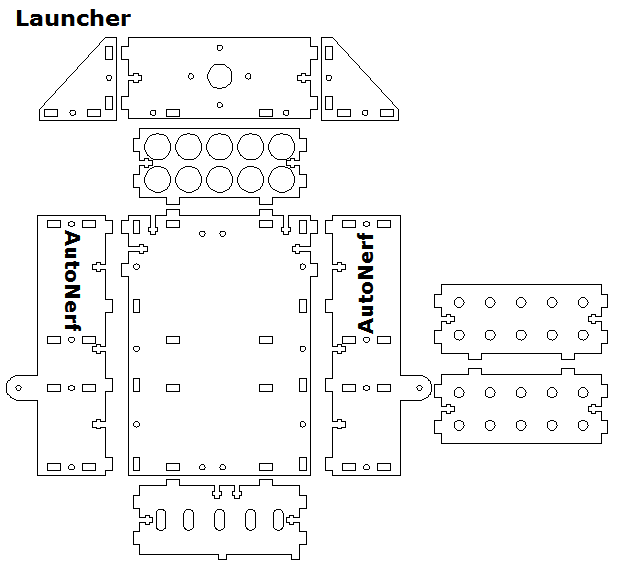
\includegraphics[scale=0.5]{figures/appendix/launcher.png}
    \caption{Ontwerp \emph{launcher}}
\end{figure}

    \chapter{Pan platform ontwerp}
\label{app:pan-platform}

\begin{figure}
    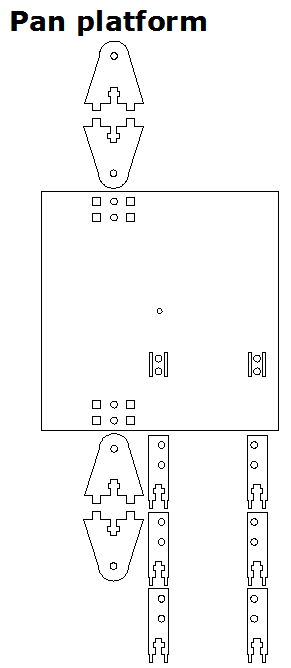
\includegraphics[scale=0.5]{figures/appendix/pan.png}
    \caption{Ontwerp \emph{pan platform}}
\end{figure}

    \chapter{Base platform ontwerp}
\label{app:base-platform}

\begin{figure}
    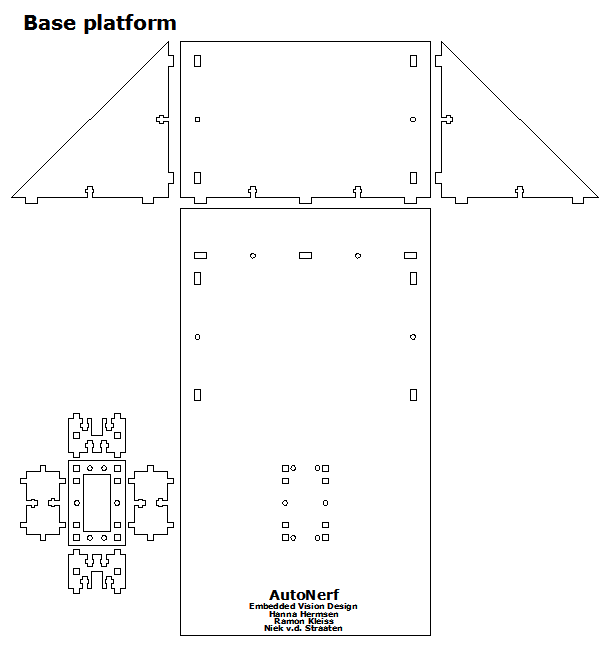
\includegraphics[scale=0.5]{figures/appendix/base.png}
    \caption{Ontwerp \emph{base platform}}
\end{figure}

    \chapter{PCB schema's}
\label{app:schematics}

\begin{figure}
    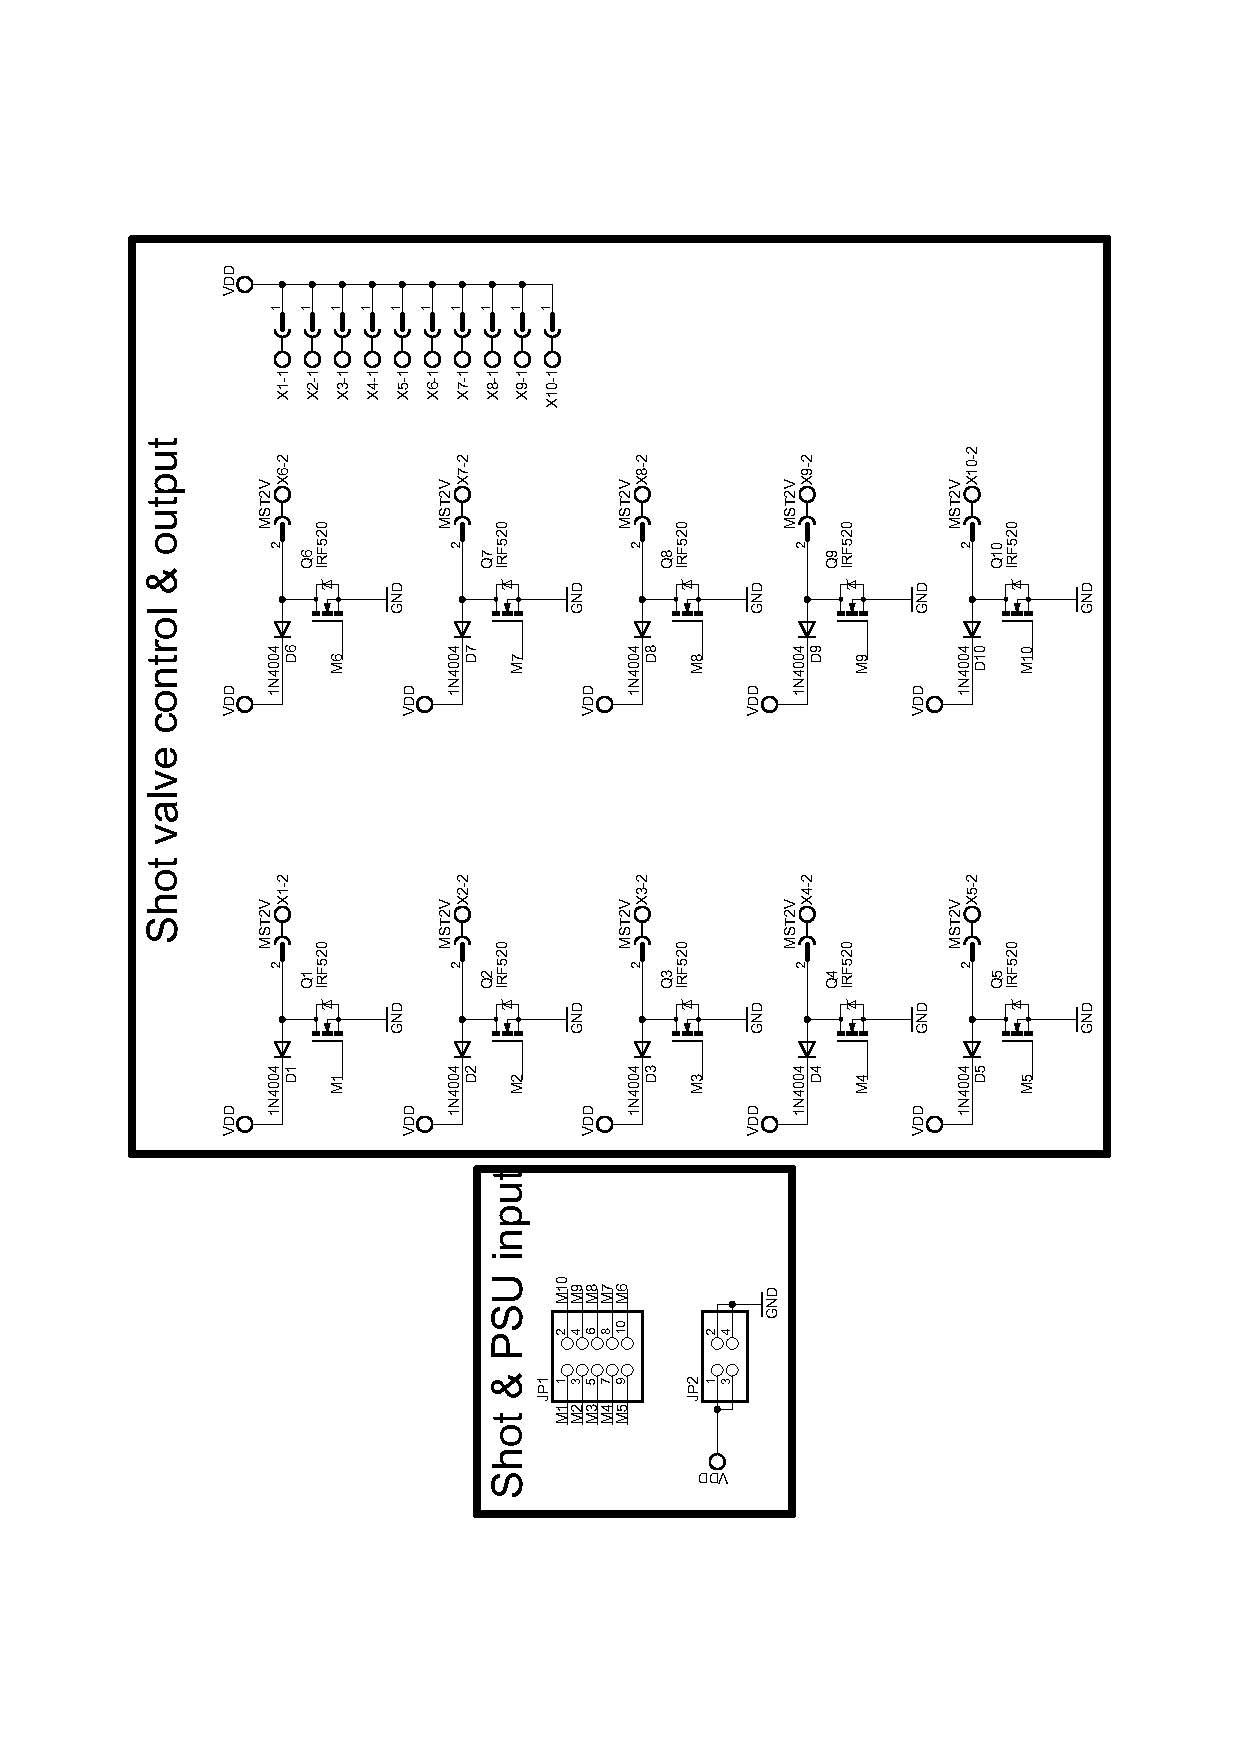
\includegraphics[scale=0.5]{figures/controller_schematic.pdf}
    \caption{Schema van \emph{controller}}
\end{figure}

\begin{figure}
    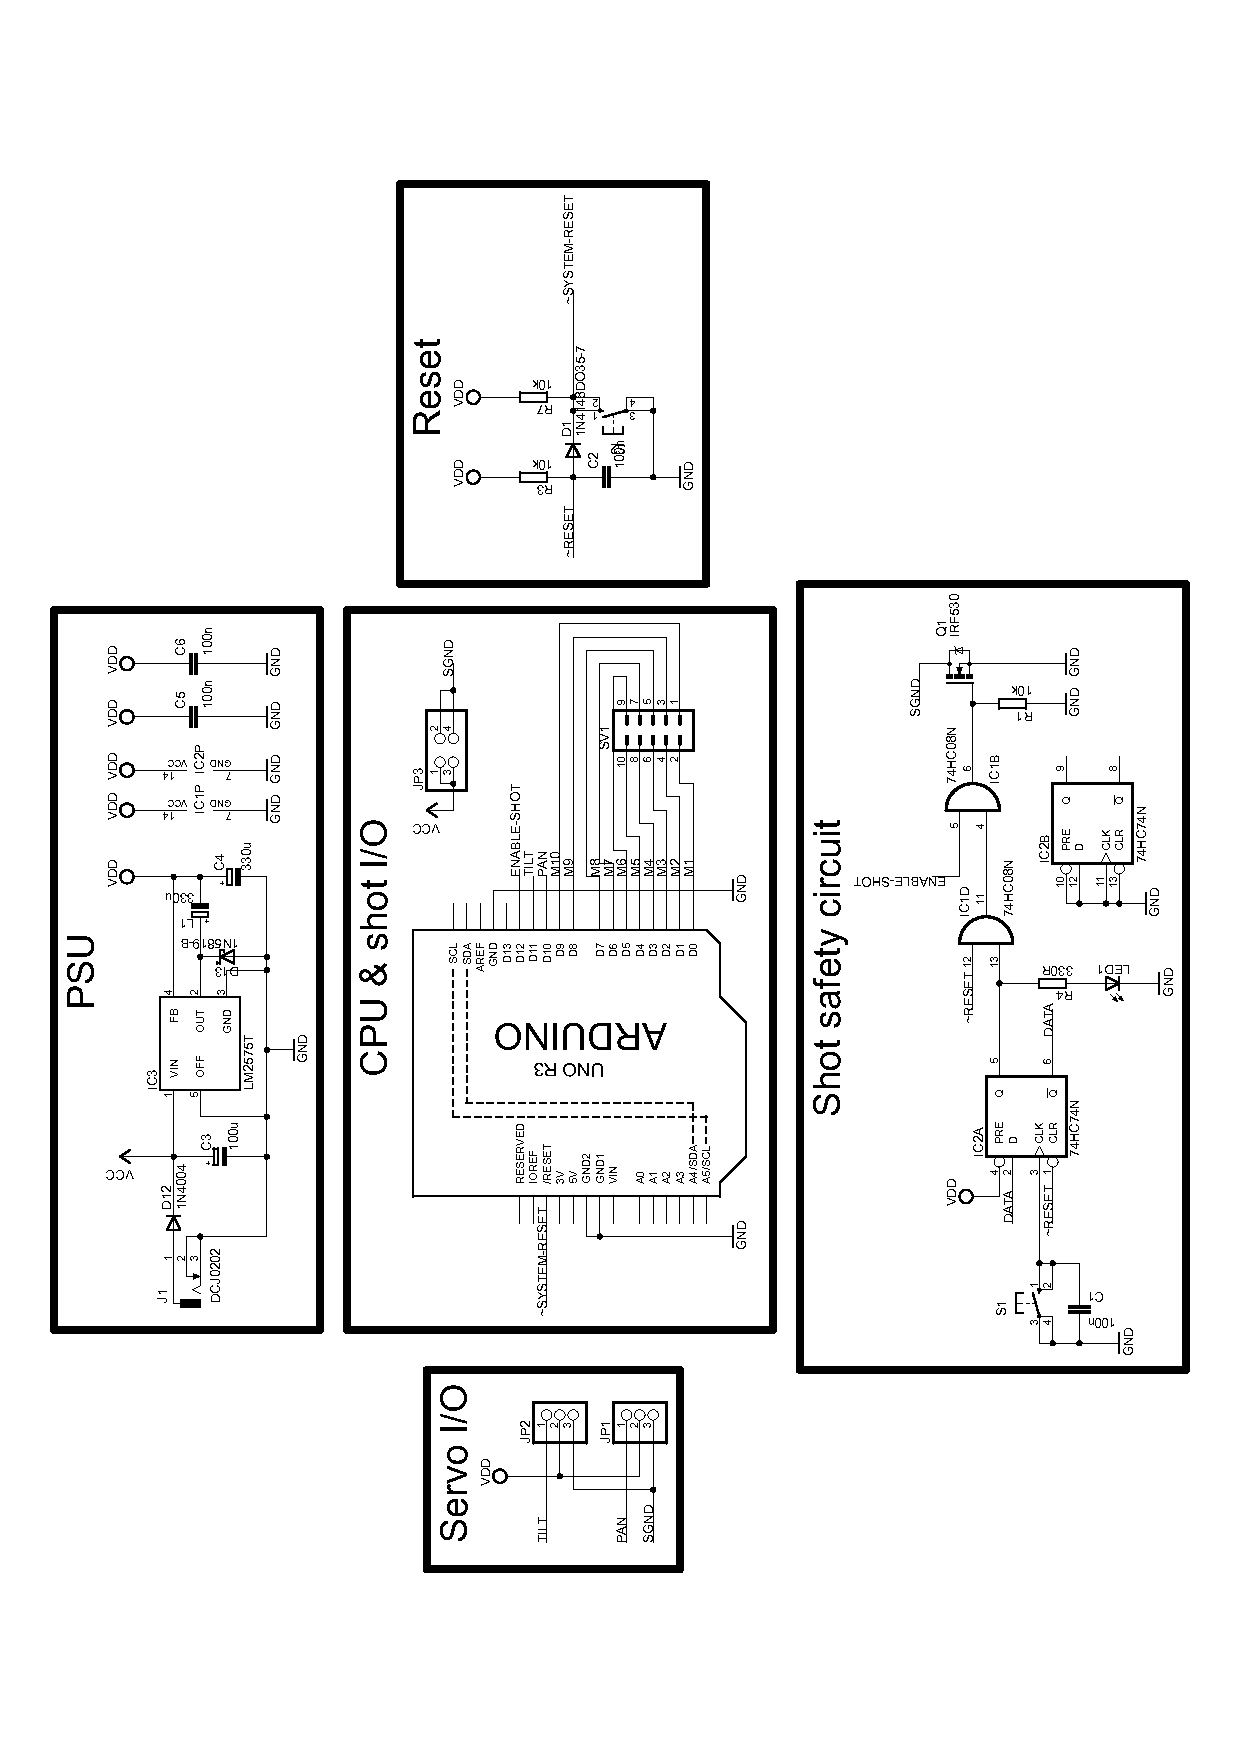
\includegraphics[scale=0.5]{figures/motherboard_schematic.pdf}
    \caption{Schema van \emph{motherboard}}
\end{figure}

    \chapter{PCB ontwerpen}
\label{app:pcb}

\begin{figure}
    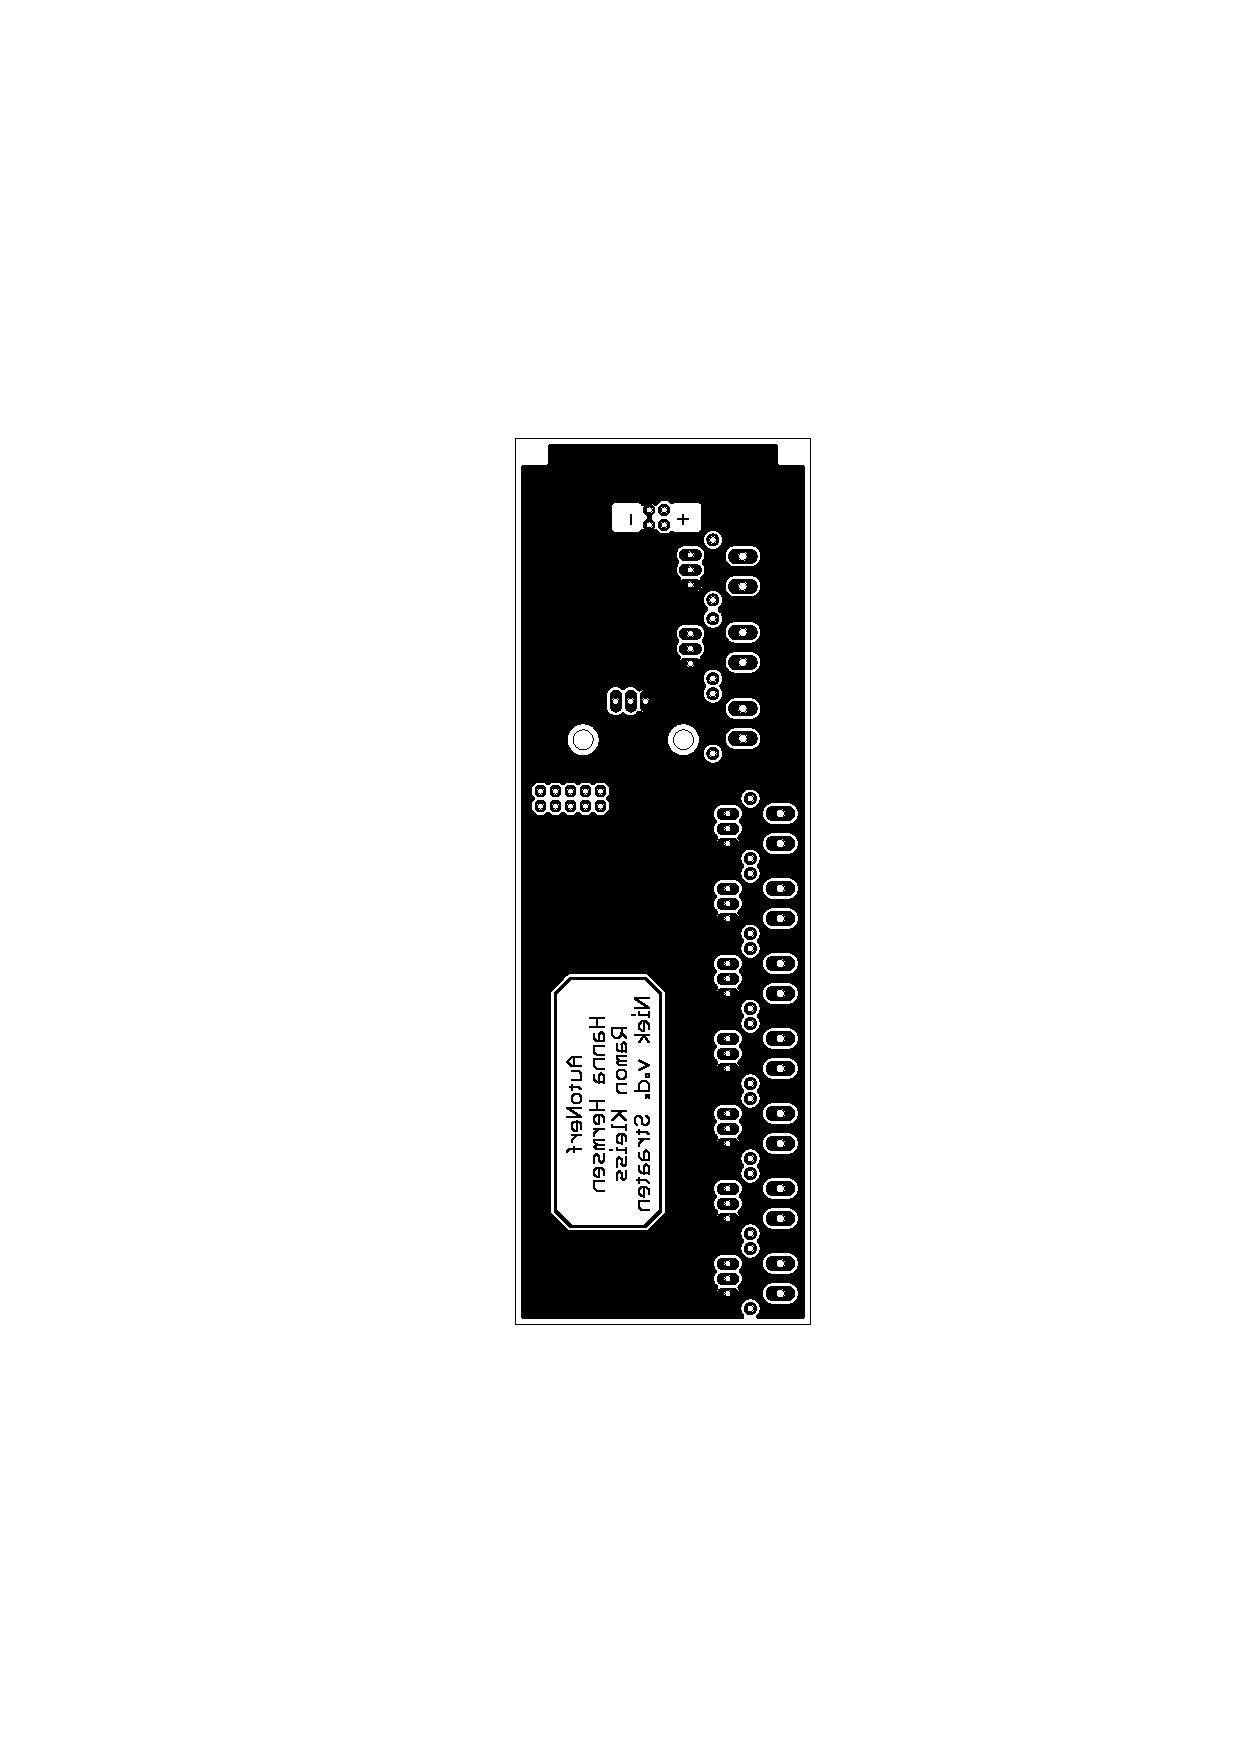
\includegraphics[scale=0.75]{figures/controller_top.pdf}
    \caption{\emph{Controller} ontwerp \emph{top}}
\end{figure}

\begin{figure}
    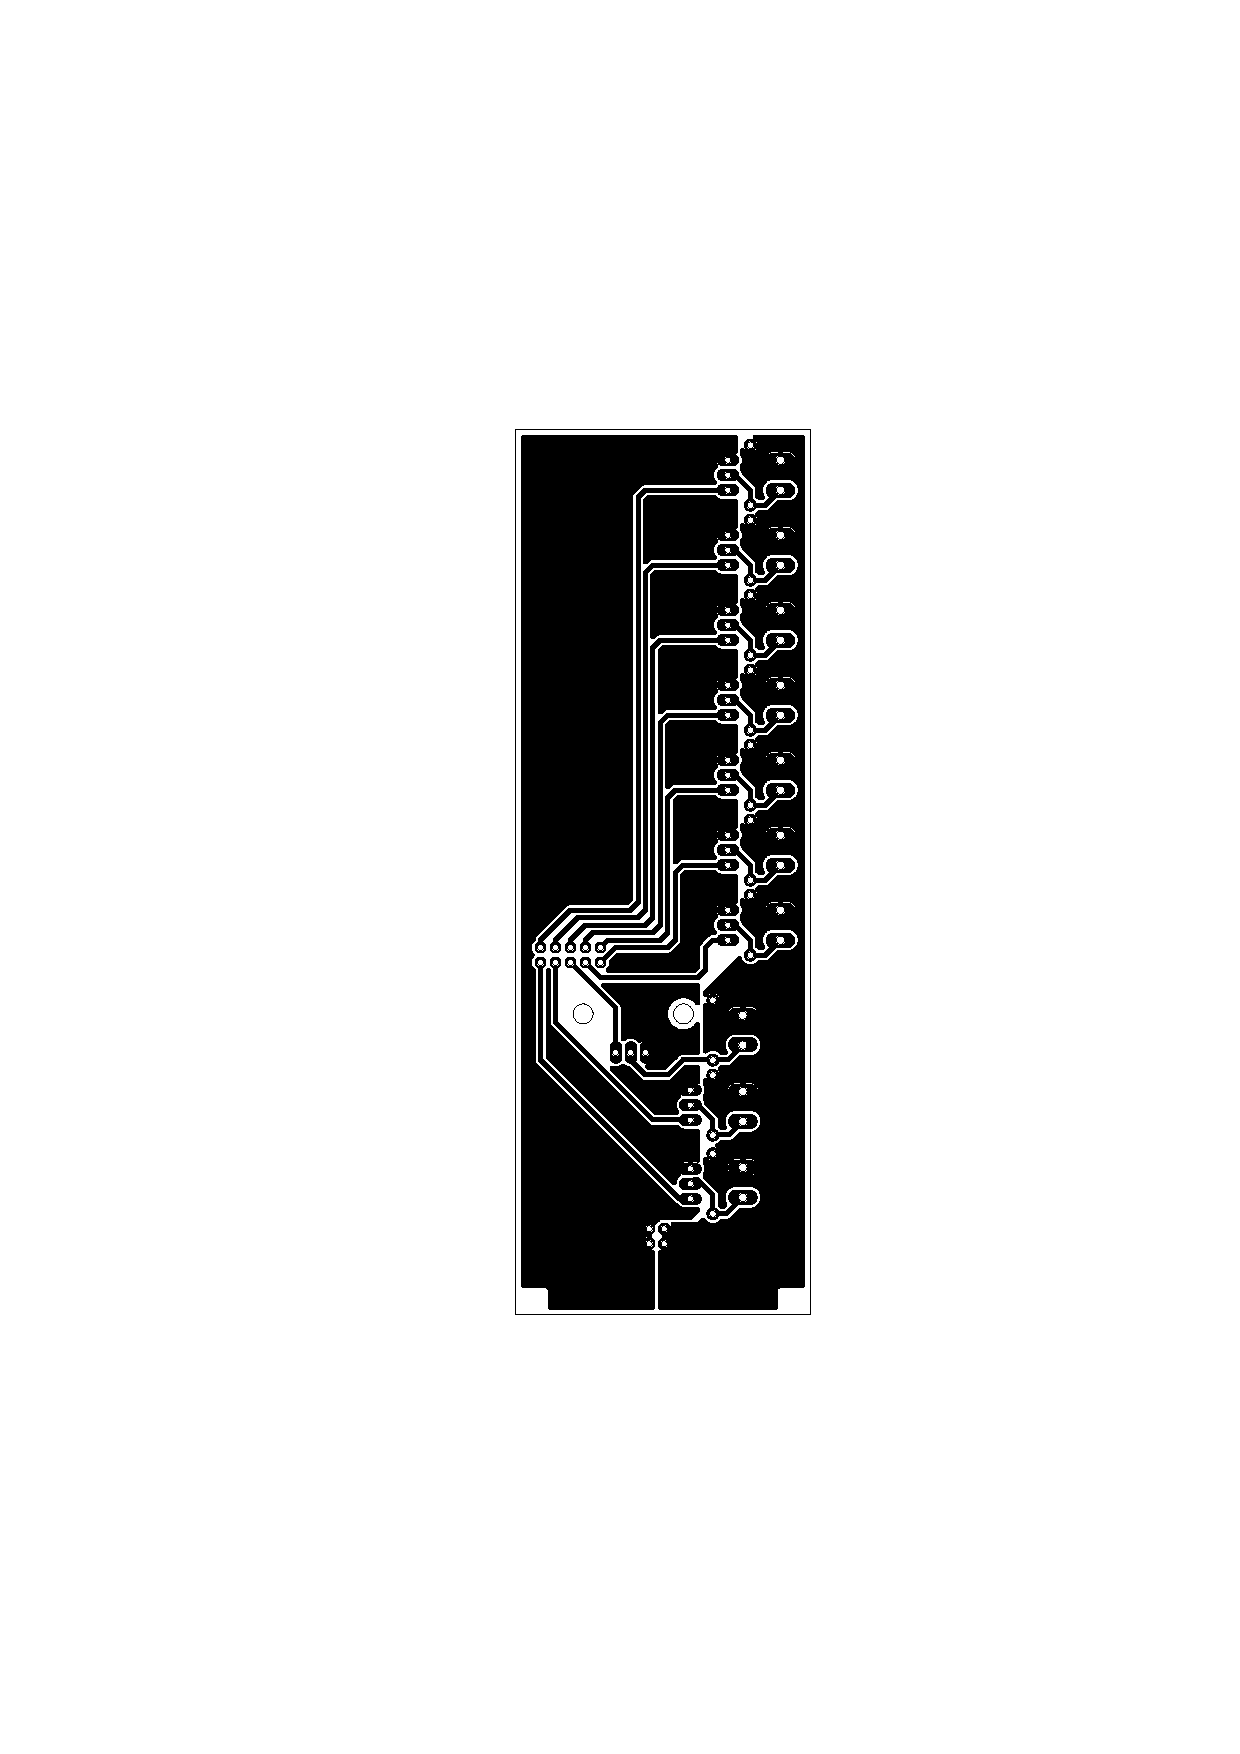
\includegraphics[scale=0.75]{figures/controller_bottom.pdf}
    \caption{\emph{Controller} ontwerp \emph{bottom}}
\end{figure}

\begin{figure}
    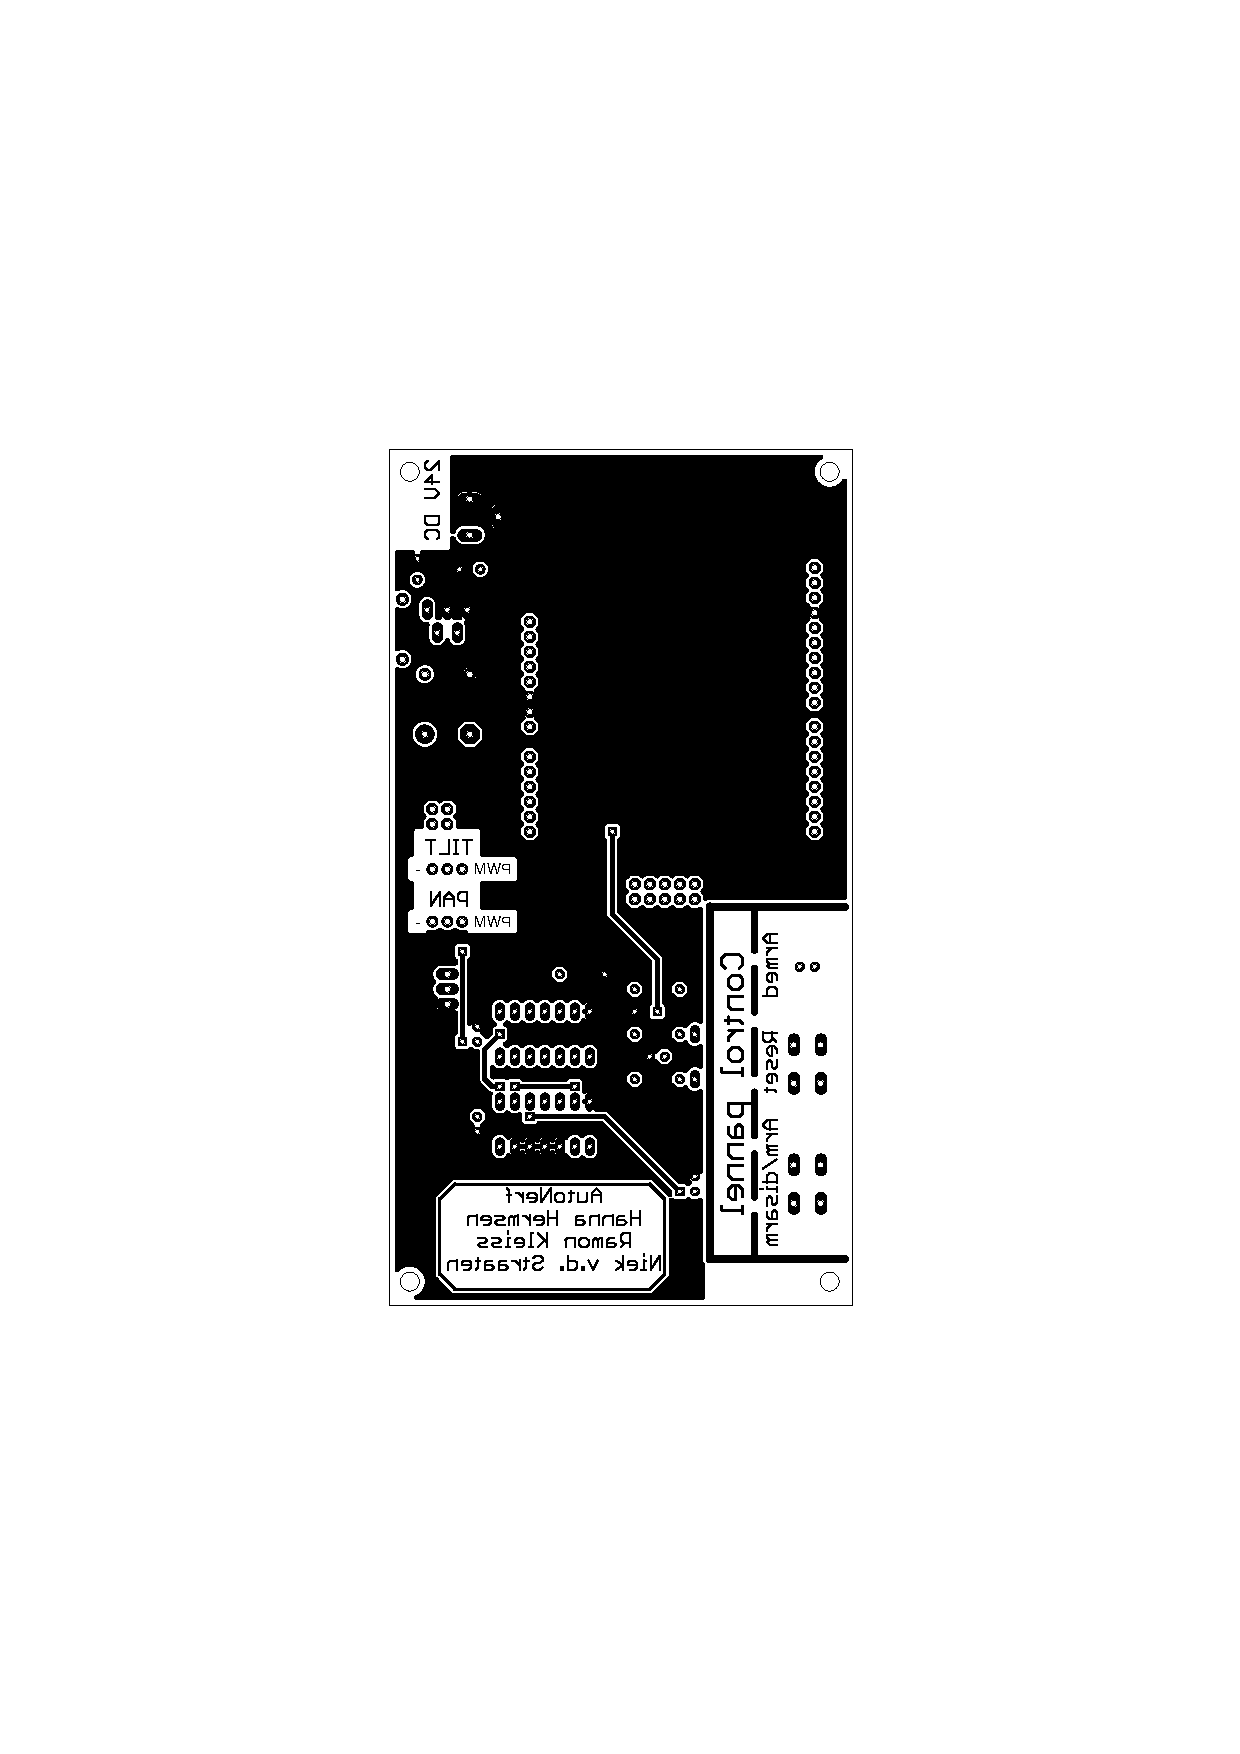
\includegraphics[scale=0.75]{figures/motherboard_top.pdf}
    \caption{\emph{Motherboard} ontwerp \emph{top}}
\end{figure}

\begin{figure}
    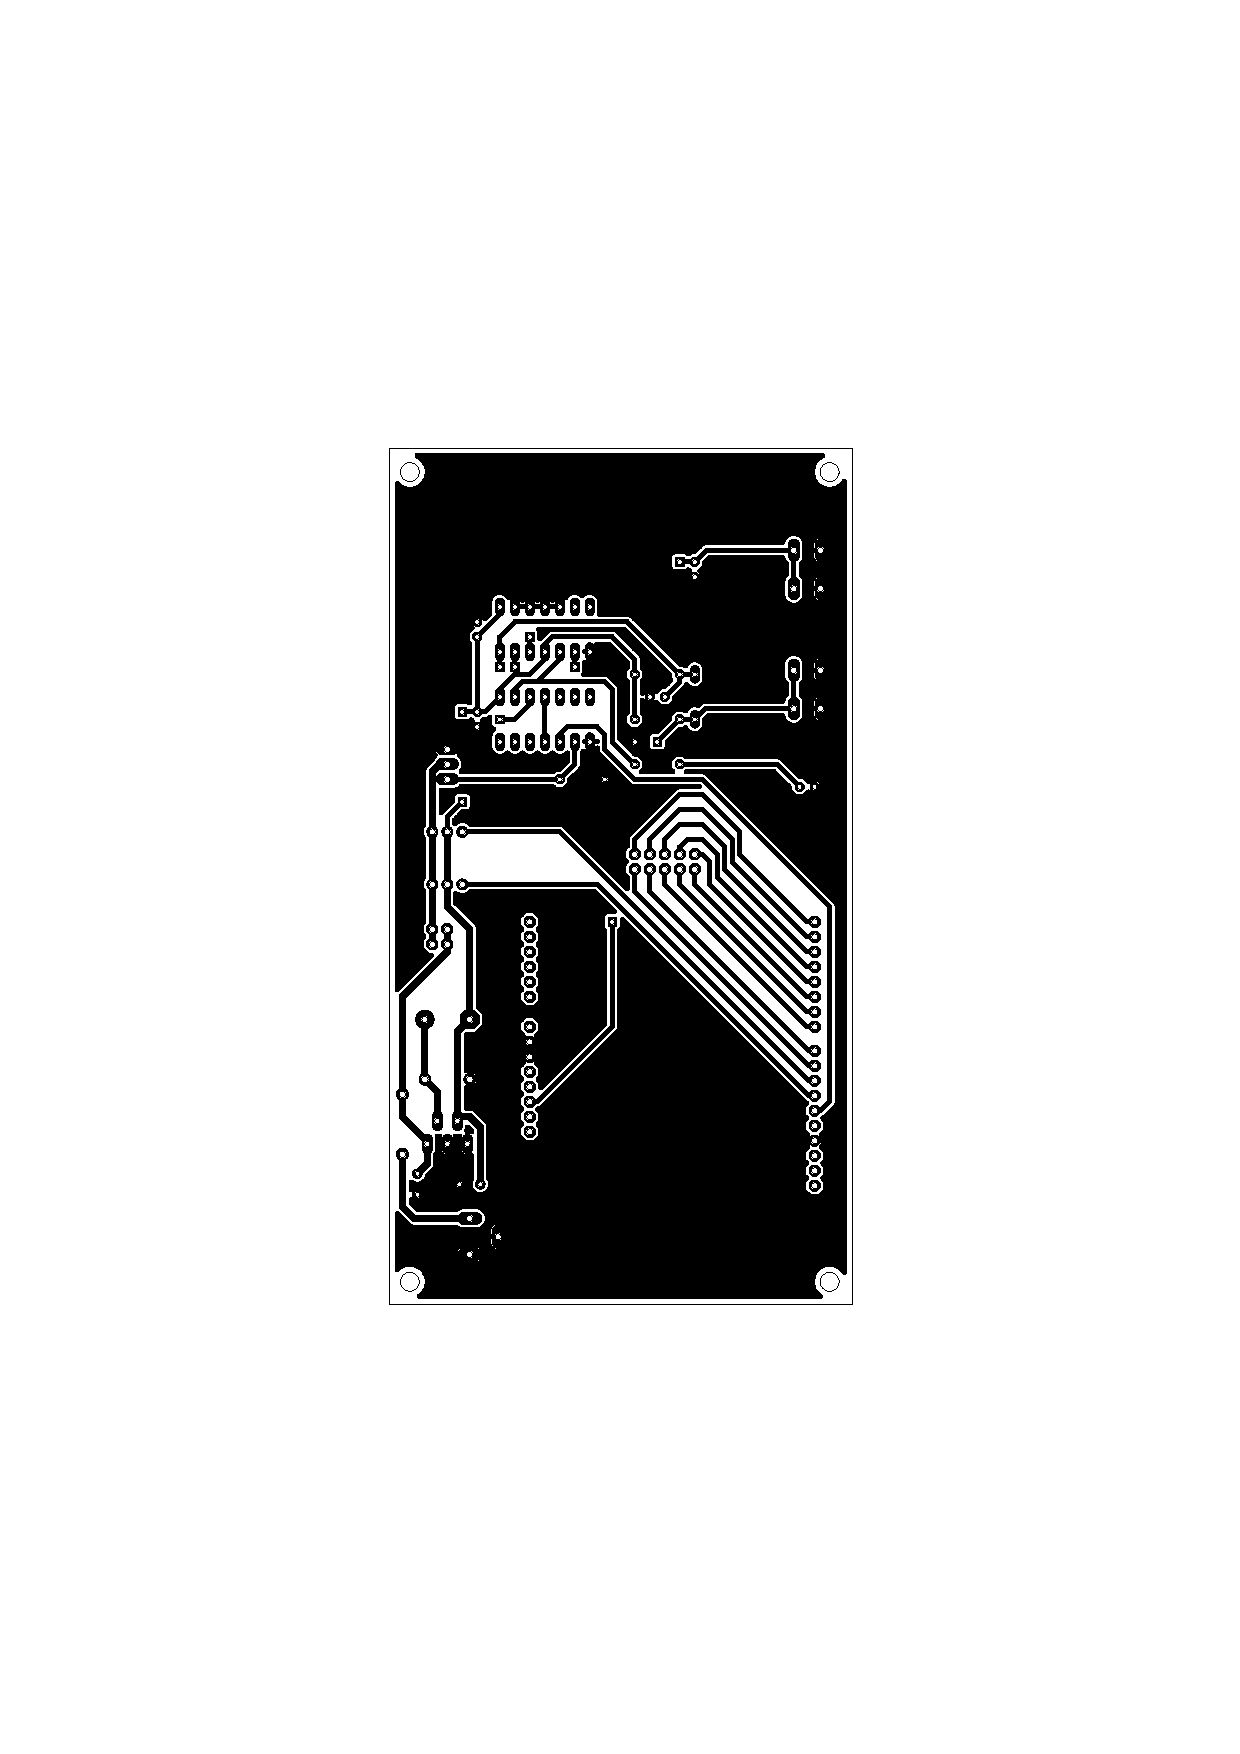
\includegraphics[scale=0.75]{figures/motherboard_bottom.pdf}
    \caption{\emph{Motherboard} ontwerp \emph{bottom}}
\end{figure}

    \end{appendices}
\end{document}
